\section{Implementation tests}

As we have implemented the restricted Boltzmann machine and the relevant hamiltonians, it would be good to know for certain that it produces meaningful result for each model. To accomplish this we will test the RBM on some small systems of the different models. This section is only meant to verify our implementation, so here we can sacrifice accuracy for less computation time. For all calculations in this section we iterate through $500$ epochs with $10000$ samples and a learning rate $\eta = 0.5$.

\subsection{The Lipkin model}

For the Lipkin model we first want to see the machine find the correct energy with no interaction between particles, single particle energy only. We make sure the machine handles increasing complexity by looking at systems with increasing size: $2$, $4$, $8$ and $16$ particles. With only single particle energy the ground state is the state where all particles occupying the lower level, which is for a N-particle system:

\begin{equation}
  E_0 = \frac{1}{2}\varepsilon N \; .
  \label{eq:Test_lipkin_single}
\end{equation}

To keep the output consistent, and make it easier to analyze, we will set

$$\varepsilon = 1$$

all throughout this section. Combining the convergence graphs into one we get:

\begin{figure}[H]
  \centering
  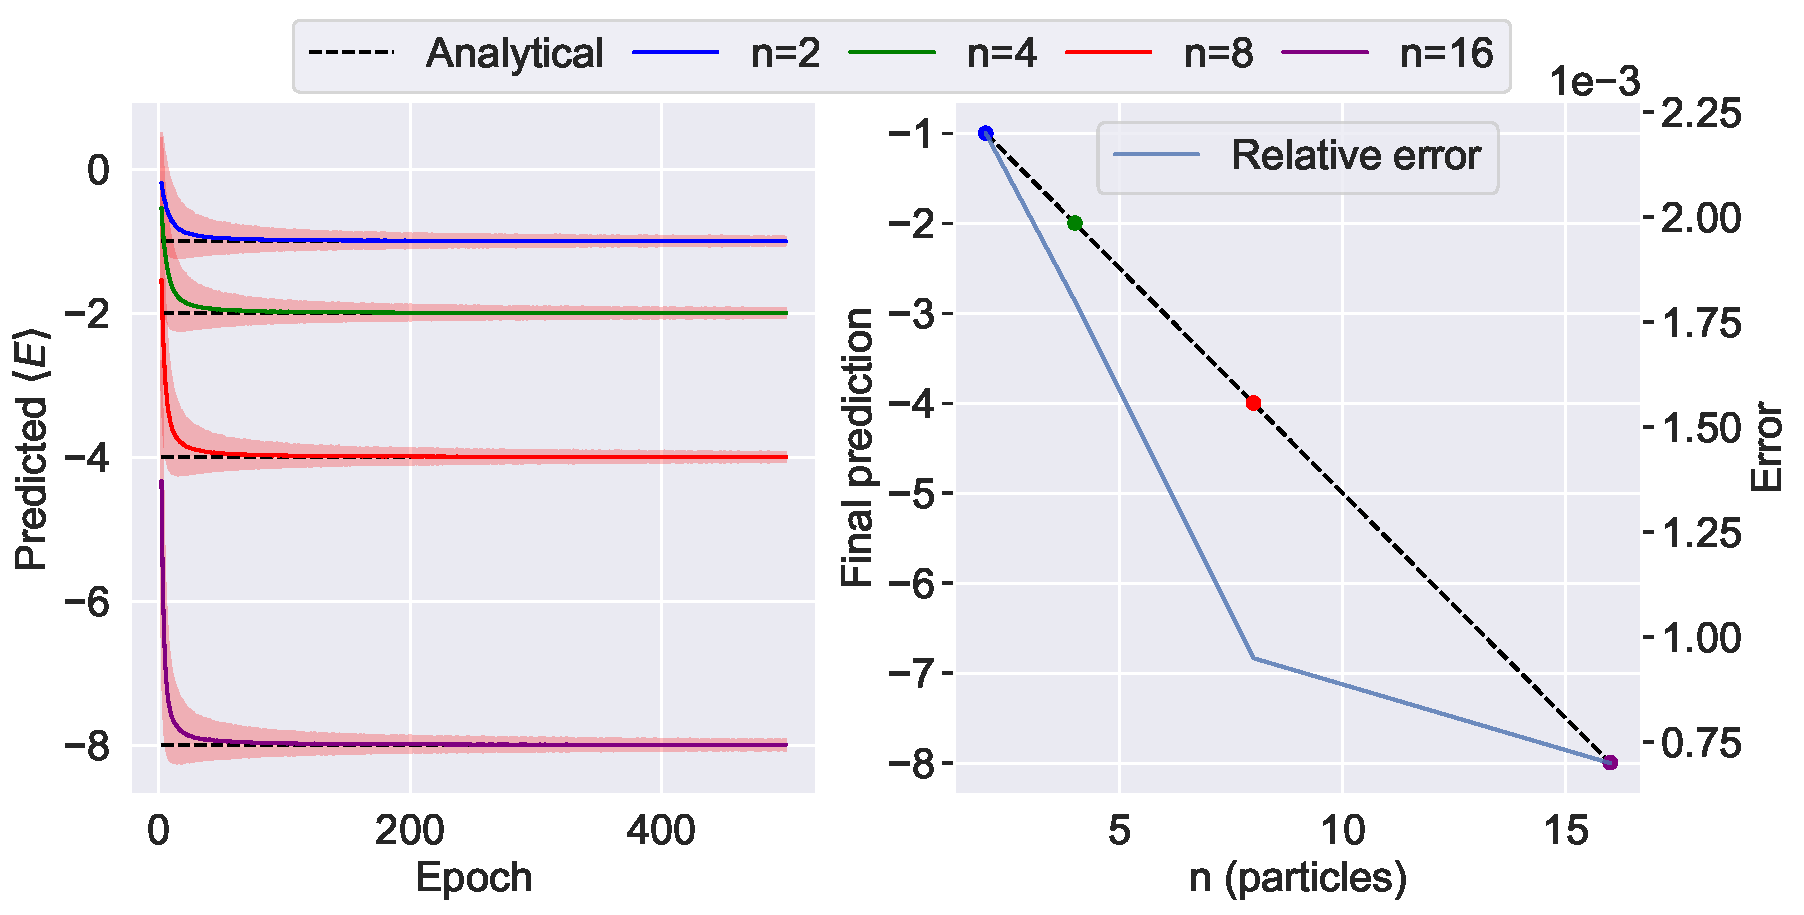
\includegraphics[width=\textwidth]{Figures/Plots/Implementation Test/Lipkin2-16.pdf}
  \caption{The predicted ground state energy for the Lipkin model without interaction and $\varepsilon = 1$. On the left is convergence plotted for each of the different number of particles and the colored area indicates the standard deviation of the local energy of the different samples. The first few data points of each convergence line is removed for readability. On the right the final output of the machine is shown with a dot for $n$ particles $2$, $4$, $8$ and $16$ together with the relative error. The dashed lines are the analytical ground state energies.}
  \label{fig:test_ground_lipkin}
\end{figure}

We see that the RBM manages to find the ground state energy for each system size. We can also see the standard deviation approaching zero. This tells us the RBM wavefunction is close to the true wavefunction because, as explained in \ref{subsec:variance_monte}:

\begin{align*} 
  \psi_{rbm} &= \psi_{true} \\
             &\Downarrow \\
  Var[&E_L] = 0 \; .
\end{align*}

The right side plot reiterates that the predicted energies follows the analytical solution, but we also see that the relative error is decreasing, although not with a factor equal to the decrease in ground state energy. Which means the error is increasing somewhat with the size of the system. Looking at the relative standard deviation:

\begin{figure}[H]
  \begin{center}
    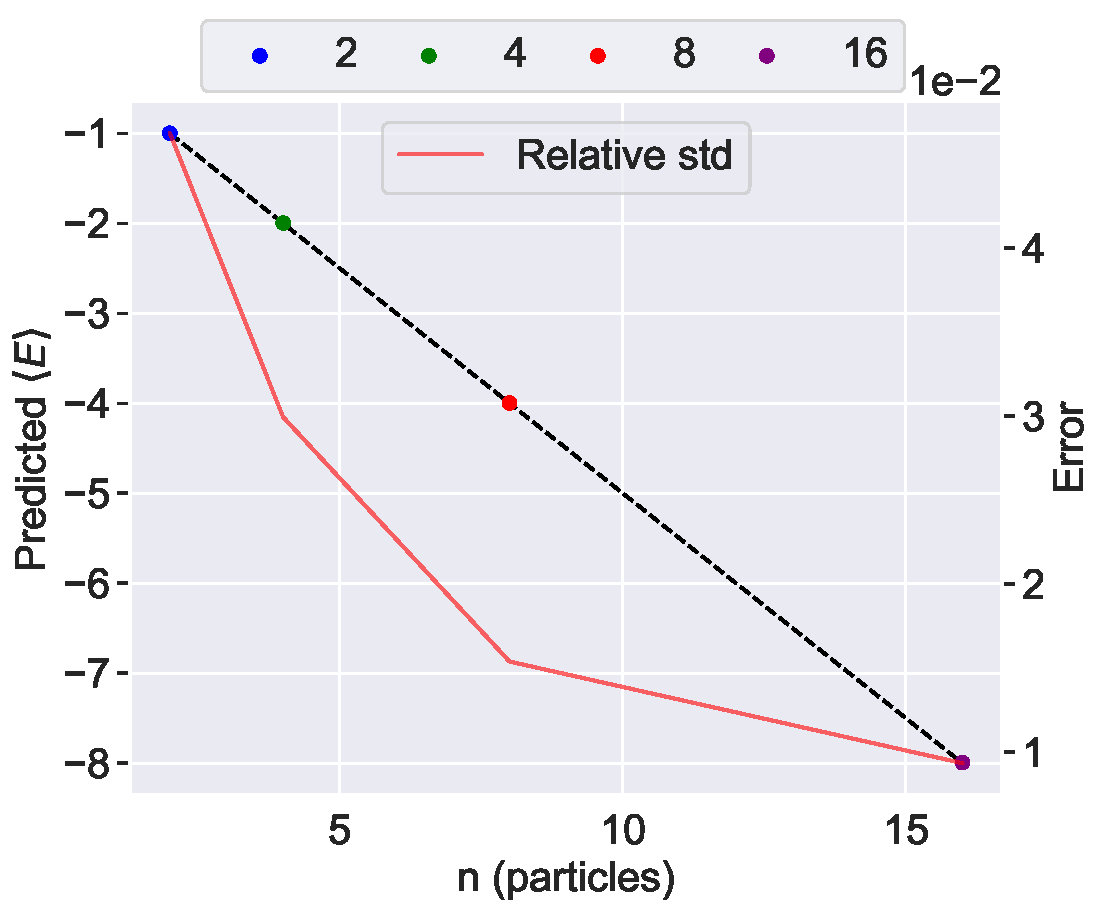
\includegraphics[width=0.7\textwidth]{Figures/Plots/Implementation Test/Lipkin_relative_std.pdf}
  \end{center}
  \caption{The found ground state energy by the restricted Boltzmann machine for the Lipkin model without interaction together with the relative standard deviation error.}
  \label{fig:Lipkin_relative_std}
\end{figure}

we can see that it also decreases with the number of particles. However, the relative standard deviation decreases more, relatively from $n=2$ to $n=16$, than the relative error does. This would indicate that the overall increase in error mostly comes from the increase in local energy of the basis states that are wrongly part of the machine state rather than a increase in the machine state's spread.
\subsection{The Ising model}

\subsection{The Pairing model}

\subsection{The Heisenberg model}

